
%\documentclass[mathserif]{beamer}
\documentclass[handout]{beamer}
%\usetheme{Goettingen}
%\usetheme{Warsaw}
\usetheme{Singapore}



%\usetheme{Frankfurt}
%\usetheme{Copenhagen}
%\usetheme{Szeged}
%\usetheme{Montpellier}
%\usetheme{CambridgeUS}
%\usecolortheme{}
%\setbeamercovered{transparent}
\usepackage[english, activeacute]{babel}
\usepackage[utf8]{inputenc}
\usepackage{amsmath, amssymb}
\usepackage{dsfont}
\usepackage{graphics}
\usepackage{cases}
\usepackage{graphicx}
\usepackage{pgf}
\usepackage{epsfig}
\usepackage{amssymb}
\usepackage{multirow}	
\usepackage{amstext}
\usepackage[ruled,vlined,lined]{algorithm2e}
\usepackage{amsmath}
\usepackage{epic}
\usepackage{epsfig}
\usepackage{fontenc}
\usepackage{framed,color}
\usepackage{palatino, url, multicol}
%\algsetup{indent=2em}
\newcommand{\factorial}{\ensuremath{\mbox{\sc Factorial}}}
\newcommand{\BIGOP}[1]{\mathop{\mathchoice%
{\raise-0.22em\hbox{\huge $#1$}}%
{\raise-0.05em\hbox{\Large $#1$}}{\hbox{\large $#1$}}{#1}}}
\newcommand{\bigtimes}{\BIGOP{\times}}
\vspace{-0.5cm}
\title{Supervised models for Twitter opinion lexicon expansion}
\vspace{-0.5cm}
\author[Felipe Bravo Márquez]{\footnotesize
%\author{\footnotesize  
 \textcolor[rgb]{0.00,0.00,1.00}{Felipe Bravo-Marquez} \\ Chief Supervisor: Bernhard Pfahringer \\  Supervisor: Eibe Frank} 
  
 
%\vspace{-0.3cm}
\institute{University of Waikato \\ Computer Science Department }

\titlegraphic{\includegraphics[scale=0.3]{../../img/waikato.png}}



\date{August 18, 2015}

\begin{document}
\begin{frame}
\titlepage


\end{frame}



\begin{frame}{Social Media}
\begin{scriptsize}
\begin{itemize}
 \item Microblogging services are increasingly being adopted by people in order to access and publish information.  
 \item \textbf{Twitter}: Massively used Microblogging platform where users post messages limited to 140 characters. 
 \item Twitter users tend to publish \textbf{personal opinions} regarding certain topics and news events. 
\end{itemize}
  \begin{figure}[h]
        	
\includegraphics[scale = 0.2]{pics/twitter.png}
        \end{figure}

\end{scriptsize}
\end{frame}



\begin{frame}{Sentiment Analysis and Social Media}
\begin{scriptsize}
\begin{itemize}
 \item Opinions are provided \textbf{freely and voluntarily} by the users in Twitter. 
 \item Analysing the sentiment underlying these opinions has important applications in product \textbf{marketing} and \textbf{politics}.
 
   \begin{figure}[h]
        	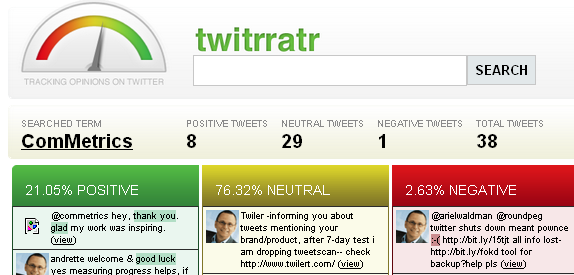
\includegraphics[scale = 0.6]{pics/tweetOpinions.png}
        \end{figure}
\end{itemize}
\end{scriptsize}




\end{frame}

\begin{frame}{Opinion Mining or Sentiment Analysis}
\begin{scriptsize}\begin{itemize}
 \item Application of \textbf{NLP} and \textbf{text mining} techniques to identify and extract subjective information from textual datasets.
\end{itemize}
\pause
\begin{block}{Sentiment Classification Problem}
  \begin{enumerate}
   \item Automatically classify a textual message to classes \textcolor[rgb]{0.00,0.00,1.00}{\textbf{positive}}, \textcolor[rgb]{1.00,0.00,0.00}{\textbf{negative}}, or \textcolor[rgb]{0.00,1.00,0.00}{\textbf{neutral}}. 
  \end{enumerate} 
\end{block}

  \begin{figure}[h]
        	
\includegraphics[scale = 0.15]{pics/sent.png}
        \end{figure}


\begin{block}{Approaches}
\begin{itemize}
\item Most methods rely on opinion lexicons.
\item An opinion lexicon is a lists of terms labelled by sentiment.
\item They are normally composed of positive and negative words such as \textcolor[rgb]{0.00,0.00,1.00}{\textbf{happy, wonderful}} and \textcolor[rgb]{1.00,0.00,0.00}{\textbf{sad, bad}}.
\end{itemize}

\end{block}

\end{scriptsize}

\end{frame}




\begin{frame}{The Twitter dialect}
\begin{scriptsize}
\begin{itemize}
 \item The words used in Twitter include many abbreviations, acronyms, and misspelled words, e.g., \textbf{lol}, \textbf{omg}, \textbf{hahaha}, \textbf{\#hatemonday}.
\item This words are \textbf{not} covered by most popular lexicons.
\item The manual creation of a Twitter-oriented opinion lexicon is a \textbf{time-consuming} task.
\end{itemize}
\end{scriptsize}




\end{frame}





\begin{frame}{Proposal}
\begin{scriptsize}
\begin{itemize}
\item We study different \textbf{supervised models} for opinion lexicon expansion for  \textbf{Twitter}.
\item The proposed models create Twitter-oriented opinion lexicons in an automatic way.
\item They rely on two resources: a \textbf{corpus of tweets} and a \textbf{seed lexicon}.
\item Each expanded word has a \textbf{probability distribution}, describing how positive, negative, and neutral it is.
\end{itemize}
\end{scriptsize}
\end{frame}




\begin{frame}{Previous work on lexicon expansion}
\begin{scriptsize}

\begin{itemize} 
 \item The expansion is normally done by exploiting \textbf{relations} between a \textbf{small seed lexicon} and \textbf{unknown words} from a \textbf{textual} resource.
\item  Two type of resources can be used: a lexical database such as \textbf{WordNet}, or a \textbf{corpus of documents}. 
\end{itemize}



\begin{figure}[h!]
	\centering
	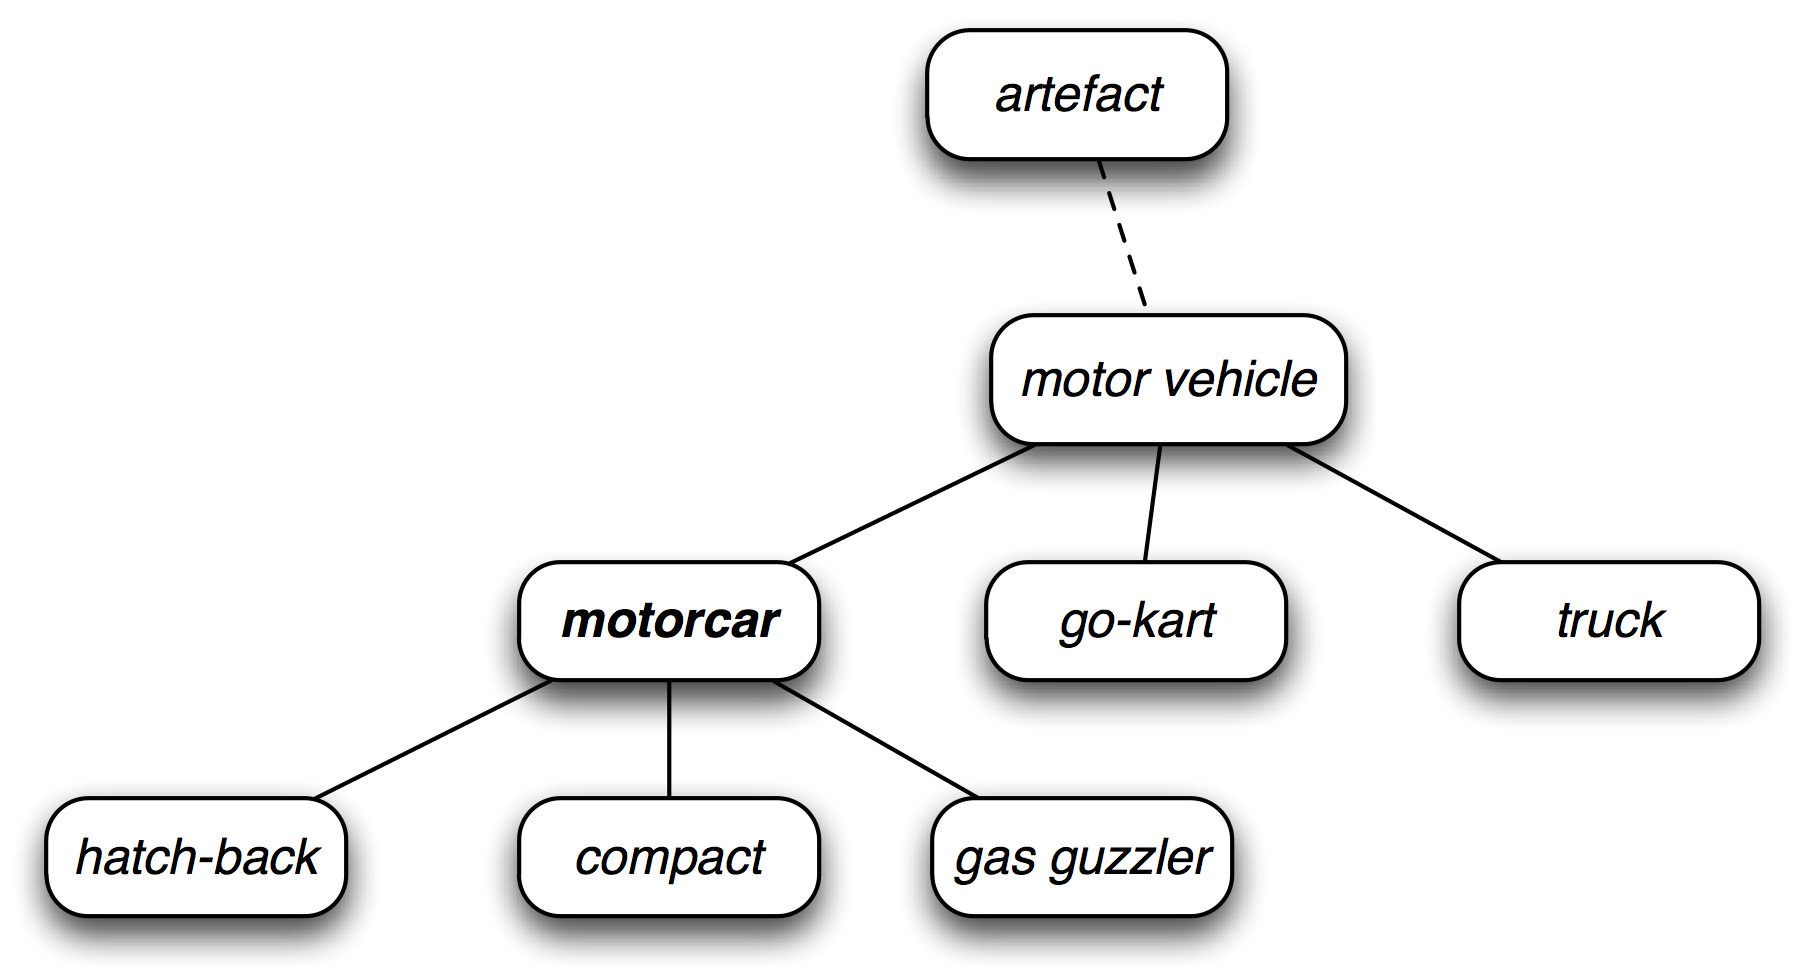
\includegraphics[scale=0.3]{pics/wordnet.png}
\end{figure}

\begin{figure}[h!]
	\centering
	
\includegraphics[scale=0.2]{pics/documents.jpg}
\end{figure}





\end{scriptsize}
\end{frame}



\begin{frame}{Lexicon expansion using WordNet}
\begin{scriptsize}

\begin{itemize} 
\item Methods based on WordNet expand the seed words using semantic relations such \textbf{synonyms} and \textbf{antonyms}, \cite{Liu2004,Kim2004}.
\item Hypothesis: synonyms have the \textbf{same} polarity and antonyms have the \textbf{opposite}.
\item In \cite{kamps2004} a \textbf{graph} was created using WordNet \textbf{adjectives} as vertices and the \textbf{synonym} relation as edges. 
\item Words are expanded by its \textbf{relative distance} from the two seed terms \textbf{good} and \textbf{bad}.
\item In \cite{Esuli2005, esuli2006} the authors take the \textbf{dictionary definitions} of the seed words to train a word-level classifier. 
\end{itemize}
\end{scriptsize}
\end{frame}






\begin{frame}{Corpus-based lexicon expansion}
\begin{scriptsize}
\begin{itemize}
\item As semantic databases cover a fixed vocabulary, they \textbf{cannot} capture domain dependent words. 
\item Corpus approaches exploit \textbf{statistical patterns} observed in document corpora. 
\item They can potentially be applied to any domain, and hence, are more suitable for \textbf{Twitter lexicon expansion}.  
\item Hartziva et. al \cite{Hatziva1997} used the  conjunction relations between adjectives.
\item Idea: adjectives connected with \textbf{and} tend to have the same polarity in the opposite way than adjectives connected with \textbf{but}.
\end{itemize}
\end{scriptsize}
\end{frame}

\begin{frame}{Corpus-based lexicon expansion (2)}
\begin{scriptsize}
\begin{itemize}
\item Turney et.al proposed an unsupervised measure called \textbf{semantic orientation} (SO) \cite{turney2003measuring} .
\item It is calculated as the difference between the point-wise mutual information \textbf{PMI} of the word with a positive and a negative seed word.

\begin{equation}
 \operatorname{PMI}(term_{1}, term_{2})= \log_{2} \left ( \frac{Pr(term_{1} \wedge term_{2})}{Pr(term_{1})Pr(term_{2})} \right )
\end{equation}

\begin{equation}\label{eq:so}
 \operatorname{SO}(word) = \operatorname{PMI}(word, ``excellent") - \operatorname{PMI}(word, ``poor")
\end{equation}

\item The PMI values are estimated by the number of \textbf{hits} returned by a search engine.

\item The resulting SO score is a numerical value whose \textbf{sign} represents the word's polarity.

\item The magnitude of the value represents the \textbf{sentiment intensity}. 


\end{itemize}
\end{scriptsize}
\end{frame}




\begin{frame}{Twitter lexicon expansion}
\begin{scriptsize}
\begin{itemize}
\item Previous Twitter lexicon generation models compute the SO between \textbf{corpus words} and tweet-level sentiment \textbf{labels}. 
\item The tweets are \textbf{automatically} labelled to polarity classes using \textbf{distant supervision} \cite{Mohammad2013, Zhou2014} or \textbf{self-training} \cite{avaya2013}. 
\item  Distant supervision methods rely on strong \textbf{sentiment clues} found in the message such as \textbf{emoticons} \cite{Mohammad2013, Zhou2014} or \textbf{hashtags}  \cite{Mohammad2013} to label the messages.
\item  Tweets where these clues are not observed are \textbf{discarded}. 
%\item In the self-training approach \cite{avaya2013} a \textbf{message-level} polarity classifier is trained from a corpus of manually labelled tweets.
%\item The classifier is used to tag a \textbf{large corpus} of \textbf{unlabelled tweets}. 
%\item The \textbf{predicted labels} and the unlabelled tweets are used to compute the SO.
\end{itemize}

\begin{table}[htbp]
\centering
\begin{tabular}{|l|l|}
\hline
positive & negative \\ \hline
:) & :( \\ 
:-) & :-( \\ 
:D & =( \\ 
=) & :'(   \\ \hline
\end{tabular}
\end{table} 


\end{scriptsize}
\end{frame}



\begin{frame}{Twitter lexicon expansion using word embeddings}
\begin{scriptsize}
\begin{itemize}

\item  Word \textbf{embeddings} are low-dimensional continuous dense word vectors trained from document corpora.

\item Most popular models are skip-gram \cite{Mikolov2013}, continuos bag-of-words \cite{Mikolov2013}, and Glove \cite{penningtonSM14}.

  \begin{figure}[h]
        	\includegraphics[scale = 0.45]{pics/cbow.png}
        \end{figure}



\item In \cite{amir2015SemEval}, they were used as \textbf{features} in a regression model for determining the association between Twitter words and \textbf{positive sentiment}. 

\item In \cite{TangCol14}  \textbf{sentiment-specific} word embeddings are proposed  by combining the skip-gram model with emoticon-annotated tweets.
\item These embeddings were used for \textbf{training} a word-level polarity classifier.
\end{itemize}
\end{scriptsize}
\end{frame}







\begin{frame}{A model based on labelled tweets}
\begin{scriptsize}
\begin{itemize}
\item We propose a \textbf{supervised framework} for \textbf{Twitter} lexicon expansion based on \textbf{sentiment-annotated tweets}.
\item The tweets are labelled in an \textbf{automatic fashion} using emoticons. 
\item Each expanded word has a \textbf{probability distribution}, describing how positive, negative, and neutral it is.
\item All the entries of the lexicon are associated with a corresponding \textbf{part-of-speech} tag.
\item This is useful for word \textbf{disambiguation} e.g., apple can be a company or a fruit.
\item These properties are inspired by \textbf{SentiWordnet}.
\end{itemize}
\end{scriptsize}

\end{frame}


\begin{frame}{Methodology}
\begin{figure}[htb]
	\centering
	 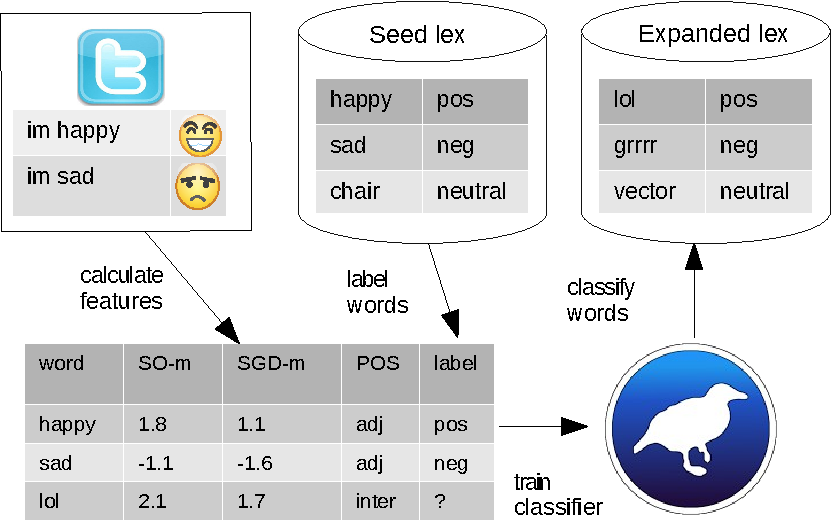
\includegraphics[scale=0.8]{diagram_crop.pdf}
	\label{fig:sosgd}
\end{figure}
\end{frame}


\begin{frame}{Ground-Truth word polarities}
\begin{scriptsize}
\begin{itemize}
\item The expansion requires a \textbf{seed lexicon} with words labelled by sentiment.
\item We create a meta-lexicon by taking the \textbf{union} of existing hand-made lexicons.
\item We discard all words where a \textbf{polarity clash} is observed.
\end{itemize}


\begin{table}[htbp]
\begin{center}
\begin{tabular}{l|c|c|c}
\hline
 & Positive & Negative & Neutral \\ \hline
AFINN & 564 & 964 & 0 \\ 
Bing Liu & 2003 & 4782 & 0 \\ 
MPQA & 2295 & 4148 & 424 \\ 
NRC-Emo & 2312 & 3324 & 7714 \\ \hline
Meta-Lex & 3730 & 6368 & 7088 \\ \hline
\end{tabular}
\end{center}
\caption{Lexicon Statistics}
\label{tab:lexstats}
\end{table}
\end{scriptsize}
\end{frame}





\begin{frame}{Obtaining labelled tweets}
\begin{scriptsize}
\begin{itemize}
\item We \textbf{require} a collection of time-stamped tweets with their corresponding \textbf{polarity labels}. 
\item Tweets can be collected from the Twitter API.
\item Tweets exhibiting \textbf{positive :)} and \textbf{negative :(} emoticons are labelled according to the emoticon's polarity.
\item We consider \textbf{two}  collections of tweets covering multiple topics: The \textbf{Edinburgh corpus} (ED), and the \textbf{Stanford Sentiment corpus} (STS).
\end{itemize}

\begin{table}[htbp]
\begin{center}
\begin{tabular}{l|c|c}
\hline
 & ED & STS \\ \hline
Positive & $1,813,705$ & $800,000$  \\ 
Negative & $324,917$ & $800,000$  \\ \hline
Total & $2,138,622$ & $1,600,000$ \\ 
\end{tabular}
\end{center}
\caption{Collection statistics}
\label{tab:colstats}
\end{table}
\end{scriptsize}

\end{frame}




\begin{frame}{Word-level Features}
\begin{scriptsize}
\begin{itemize}
\item To train the word-level classifier we need to \textbf{calculate features} from each word found in the collection of tweets.
\item Our features exploit the \textbf{temporal structure} of the collection of labelled tweets.
\item Tweets are lowercased, tokenised and POS-tagged.

\item We prepend a \textbf{POS-tag} prefix to each word in order to differentiate \textbf{homographs} exhibiting different POS-tags.

\item We create two types of \textbf{time-series} for each word: the \textbf{Stochastic Gradient Descent} (SGD) series, and the \textbf{Semantic Orientation} (SO) series.

\end{itemize}
\end{scriptsize}

\end{frame}

\begin{frame}{The SGD time-series }
\begin{scriptsize}
\begin{itemize}
\item  This time-series is calculated by incrementally training a \textbf{linear support vector machine} from the collection of labelled tweets.
\item We use \textbf{stochastic gradient descent} (SGD) online learning process.
\begin{equation}\label{eq:sgd}
\frac{\lambda}{2}||w||^2+\sum [1- y (\mathbf{xw} +b) ]_{+}.
\end{equation}
\item The weights of this linear model correspond to POS-tagged words and are updated in an \textbf{incremental fashion}.
\item  The model's weights determine how strongly the presence of a word \textbf{influences} the prediction of \textbf{polarity} classes.
\item We use \textbf{time windows} of $1,000$ examples.  

\end{itemize}
\end{scriptsize}

\end{frame}


\begin{frame}{The SO time-series }
\begin{scriptsize}
\begin{itemize}
\item  The second time-series corresponds to the \textbf{accumulated semantic orientation} (SO).
\item It is based on the \textbf{point-wise mutual information} measure.

\begin{eqnarray}
 \operatorname{SO}(w) & = & \operatorname{PMI}(w,\text{pos})- \operatorname{PMI}(w,\text{neg}) \\ \nonumber
  & = & \operatorname{log_2} \left( \frac{\Pr(w,pos)}{\Pr(w) \times \Pr(pos)} \right) -  \operatorname{log_2} \left( \frac{\Pr(w,neg)}{\Pr(w) \times \Pr(neg)} \right) \\ \nonumber
 & = & \operatorname{log_2} \left( \frac{\Pr(w,pos)\times \Pr(neg)}{\Pr(pos) \times \Pr(w,neg)} \right)
\end{eqnarray}



\begin{equation}\label{eq:so}
 \operatorname{SO}(w) = log_2 \left( \frac{\operatorname{count}(w \wedge y=1) \times \operatorname{count}(y=-1)}{\operatorname{count}(w\wedge y=-1) \times \operatorname{count}(y=1)}\right)
\end{equation}

\item We use time windows of $1,000$ examples and the \textbf{Laplace} correction to avoid the zero-frequency problem. 


\end{itemize}
\end{scriptsize}

\end{frame}


\begin{frame}{Word-level Time-Series}
\begin{scriptsize}
\begin{figure}[htb]
\begin{center}
\begin{tabular}{c}
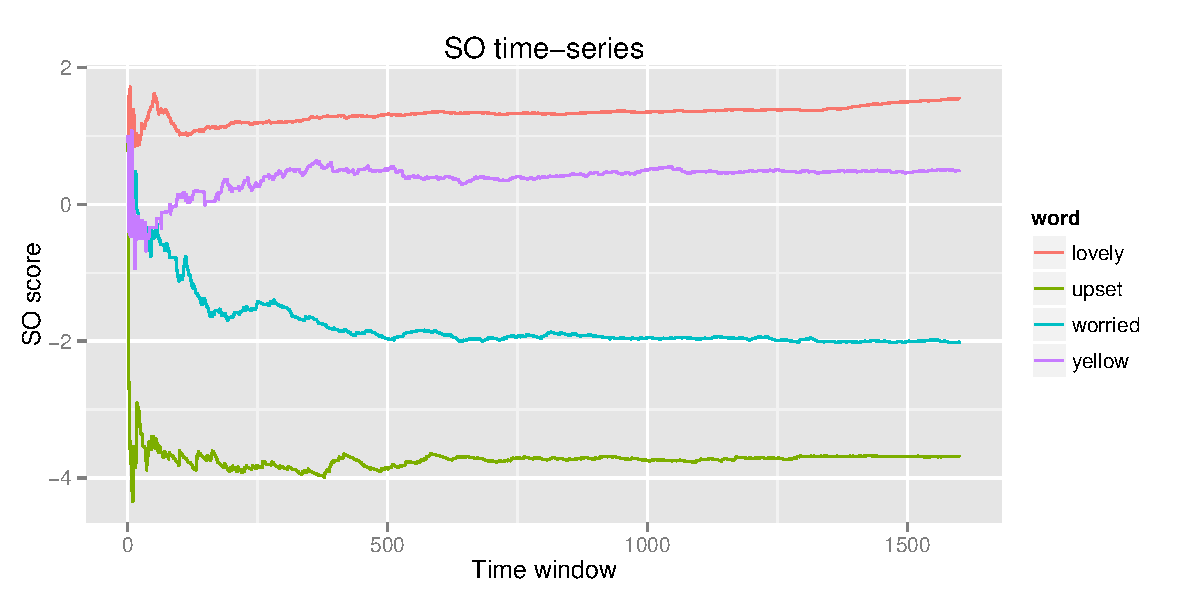
\includegraphics[scale=0.4]{../SOseries.pdf} \\
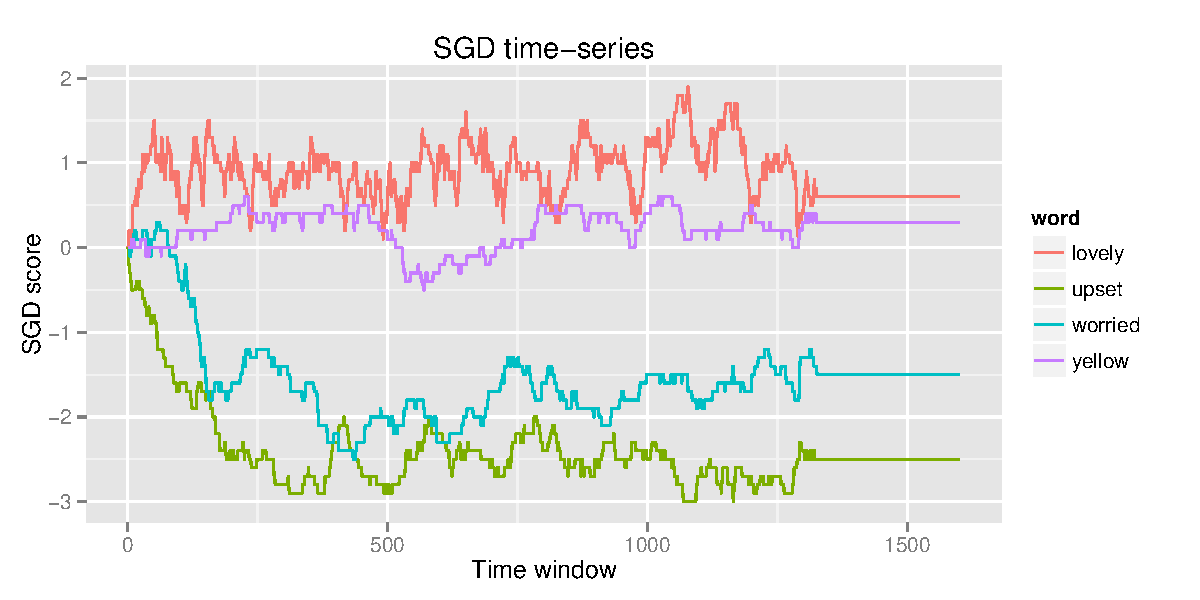
\includegraphics[scale=0.4]{../SGDseries.pdf}\\
\end{tabular}
\caption{Word-level time-series.}
\label{fig:timeseries}
\end{center}
\end{figure}
\end{scriptsize}

\end{frame}



\begin{frame}{Word-level Features}
\begin{scriptsize}
\begin{itemize}
\item We extract word-level \textbf{attributes} from both SGD and SO time-series.
\begin{table}[htbp]
\footnotesize
\begin{center}
\begin{tabular}{l|l}
\hline
Feature & Description \\ \hline
mean &  The mean of the time-series. \\ 
trunc.mean &  The truncated mean of the time-series. \\ 
median &  The median of the time-series \\ 
last.element &  The last observation of the time-series.\\ 
sd &  The standard deviation of the time-series . \\ 
iqr &  The inter-quartile range. \\ 
sg &  The fraction of times the time-series changes its sign. \\ 
sg.diff &  The sg value for the  differenced time-series. \\ \hline
\end{tabular}
\end{center}
\caption{Time-series features}
\label{tab:feat}
\end{table}

\item We also include the POS-tag of the word as a nominal attribute.

\item To create training data for machine learning, all the words \textbf{matching} the metalexicon are \textbf{labelled} according to the lexicon's polarities.

\end{itemize}
\end{scriptsize}

\end{frame}


\begin{frame}{Training data example}
\begin{scriptsize}
\begin{table}[htb]
\scriptsize
\centering
\begin{tabular}{l|llll}
  \hline
Attribute & A-lovely & A-yellow & A-upset & V-worried \\ 
  \hline
sgd.last &  0.6 &  0.3 & -2.5 & -1.5 \\ 
  sgd.mean &  0.9 &  0.2 & -2.4 & -1.6 \\ 
  sgd.trunc.mean &  0.9 &  0.2 & -2.5 & -1.6 \\ 
  sgd.median &  0.9 &  0.3 & -2.5 & -1.6 \\ 
  sgd.sd & 0.3 & 0.2 & 0.5 & 0.5 \\ 
  sgd.sg & 0.0 & 0.0 & 0.0 & 0.0 \\ 
  sgd.sg.diff & 0.2 & 0.0 & 0.1 & 0.0 \\ 
  sgd.iqr & 0.5 & 0.3 & 0.3 & 0.3 \\ 
  so.last &  1.5 &  0.5 & -3.7 & -2.0 \\ 
  so.mean &  1.3 &  0.4 & -3.7 & -1.8 \\ 
  so.trunc.mean &  1.3 &  0.4 & -3.7 & -1.9 \\ 
  so.median &  1.3 &  0.5 & -3.7 & -1.9 \\ 
  so.sd & 0.1 & 0.2 & 0.2 & 0.4 \\ 
  so.sg & 0.0 & 0.0 & 0.0& 0.0 \\ 
  so.sg.diff & 0.5 & 0.4 & 0.4 & 0.4 \\ 
  so.iqr & 0.1 & 0.1 & 0.1 & 0.1 \\ 
  pos.tag & adjective & adjective & adjective & verb \\ \hline
  label & positive & neutral & negative & negative \\ 
   \hline
\end{tabular}
\caption{Word-level feature example.}
\label{fig:featex}
\end{table}
\end{scriptsize}

\end{frame}


\begin{frame}{Feature Visualisation}
\begin{scriptsize}
\begin{figure}[htb]
	\centering
	 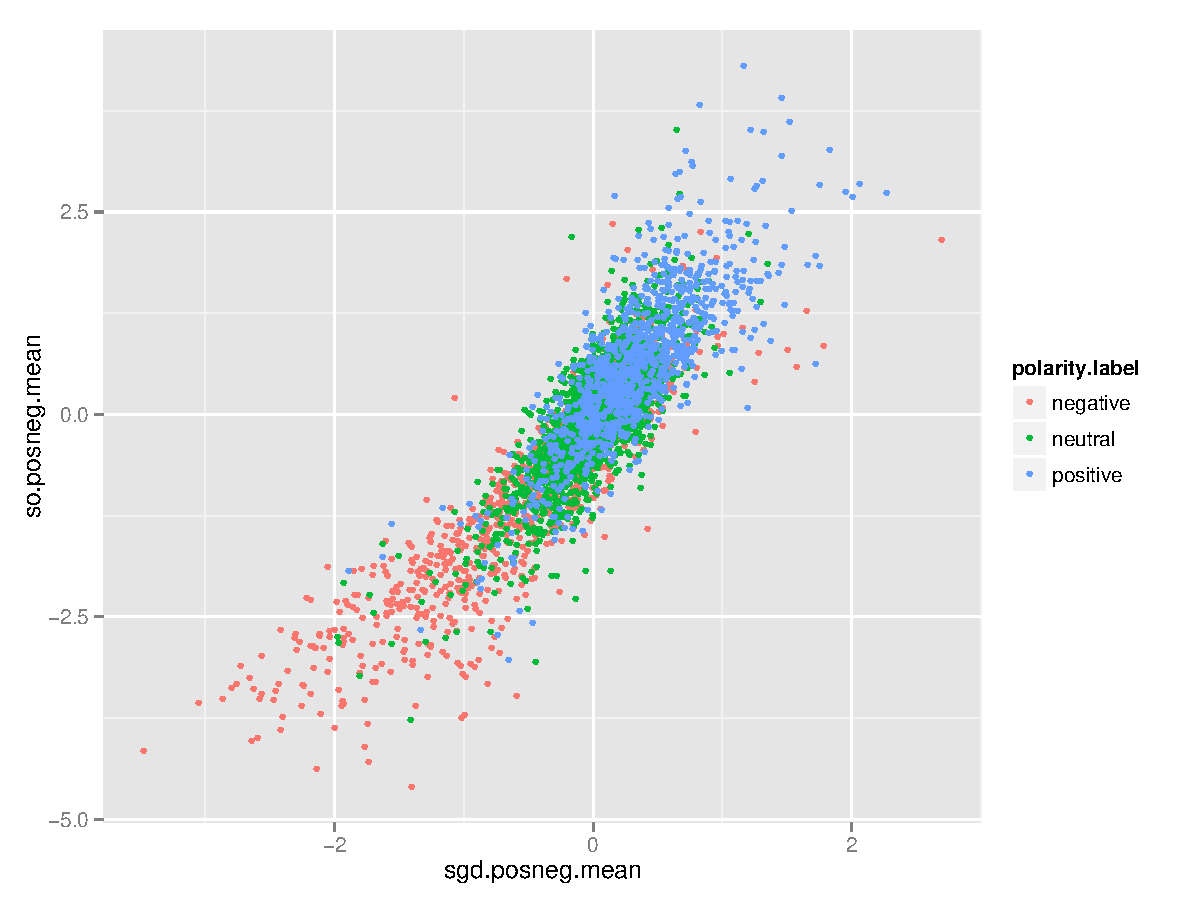
\includegraphics[width=7.5cm,height=6cm]{../SGDSO.pdf}
	\caption{SO vs SGD scatterplot.}
	\label{fig:sosgd}
\end{figure}
\end{scriptsize}

\end{frame}


\begin{frame}{Feature Visualisation (2)}
\begin{scriptsize}
\begin{figure}[ht]
\begin{center}
\begin{tabular}{c}
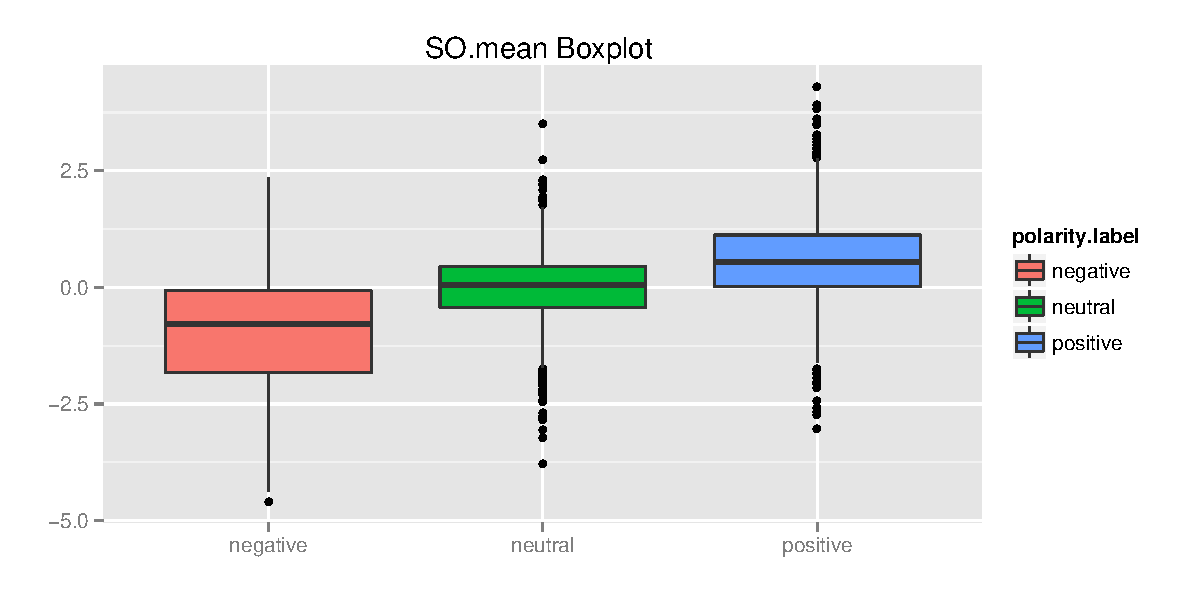
\includegraphics[scale=0.4]{../SObox.pdf}\\
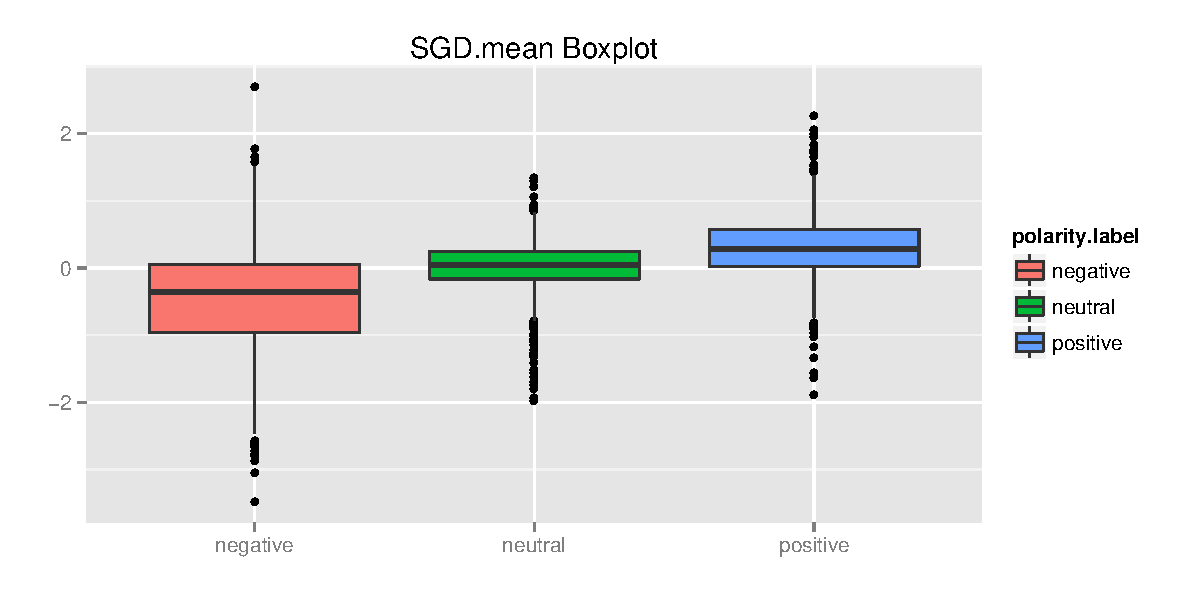
\includegraphics[scale=0.4]{../SGDbox.pdf}
\end{tabular}
\caption{SO and SGD  Boxplots.}
\label{fig:box}
\end{center}
\end{figure} 
\end{scriptsize}
\end{frame}




\begin{frame}{Word-level Classification Results using RBF SVMs}
\footnotesize
\begin{table}[!htb]
\begin{center}
\begin{tabular}{l|l|l}
\hline \hline
\multicolumn{ 3}{c}{Weighted AUC } \\ \hline \hline
Dataset & SO & ALL \\ \hline
%ED-Neutrality & 0.62 $\pm$ 0.02 &  \textbf{0.65 $\pm$ 0.02} $\circ$ \\ 
%ED-PosNeg & 0.74 $\pm$ 0.03 & \textbf{0.75 $\pm$ 0.03} \\ 
ED-Polarity & 0.62 $\pm$ 0.02 &  \textbf{0.65 $\pm$0.02} $\circ$ \\ 
%STS-Neutrality & 0.63 $\pm$ 0.02 & \textbf{0.67 $\pm$ 0.02} $\circ$ \\ 
%STS-PosNeg & \textbf{0.77 $\pm$ 0.03} &  \textbf{0.77 $\pm$ 0.03} \\ 
STS-Polarity & 0.64 $\pm$ 0.02 & \textbf{0.66 $\pm$ 0.01} $\circ$   \\ \hline 
\hline \hline
\multicolumn{ 3}{c}{Kappa} \\ \hline \hline
Dataset & SO & ALL \\ \hline
%ED-Neutrality & 0.62 $\pm$ 0.02 &  \textbf{0.65 $\pm$ 0.02} $\circ$ \\ 
%ED-PosNeg & 0.74 $\pm$ 0.03 & \textbf{0.75 $\pm$ 0.03} \\ 
ED-Polarity & 0.28 $\pm$ 0.04 &  \textbf{0.33 $\pm$0.04} $\circ$ \\ 
%STS-Neutrality & 0.63 $\pm$ 0.02 & \textbf{0.67 $\pm$ 0.02} $\circ$ \\ 
%STS-PosNeg & \textbf{0.77 $\pm$ 0.03} &  \textbf{0.77 $\pm$ 0.03} \\ 
STS-Polarity & 0.31 $\pm$ 0.04 & \textbf{0.35 $\pm$ 0.03} $\circ$   \\ \hline 


\end{tabular}
\end{center}
\caption{World-level classification performance.} 
\label{tab:classres}
\end{table}


\end{frame}


\begin{frame}{Expanded Lexicon}
\begin{table}[htbp]
\scriptsize
\begin{tabular}{l|l|l|r|r|r}
\hline
word & POS & label & negative & neutral& positive \\ \hline
alrighty & interjection & positive & 0.021 & 0.087 & 0.892 \\ 
boooooo & interjection & negative & 0.984 & 0.013 & 0.003 \\ 
lmaoo & interjection & positive & 0.19 & 0.338 & 0.472 \\ 
french & adjective & neutral & 0.357 & 0.358 & 0.285 \\ 
handsome & adjective & positive & 0.007 & 0.026 & 0.968 \\ 
saddest & adjective & negative & 0.998 & 0.002 & 0 \\ 
same & adjective & negative & 0.604 & 0.195 & 0.201 \\ 
anniversary & common.noun & neutral & 0.074 & 0.586 & 0.339 \\ 
tear & common.noun & negative & 0.833 & 0.124 & 0.044 \\ 
relaxing & verb & positive & 0.064 & 0.244 & 0.692 \\ 
wikipedia & proper.noun & neutral & 0.102 & 0.644 & 0.254 \\ \hline
\end{tabular}
\caption{Expanded words example.}
\label{tab:expwords}
\end{table}
\end{frame}


\begin{frame}{Expanded Lexicon (2)}
\begin{figure}[ht]
\begin{center}
\begin{tabular}{cc}
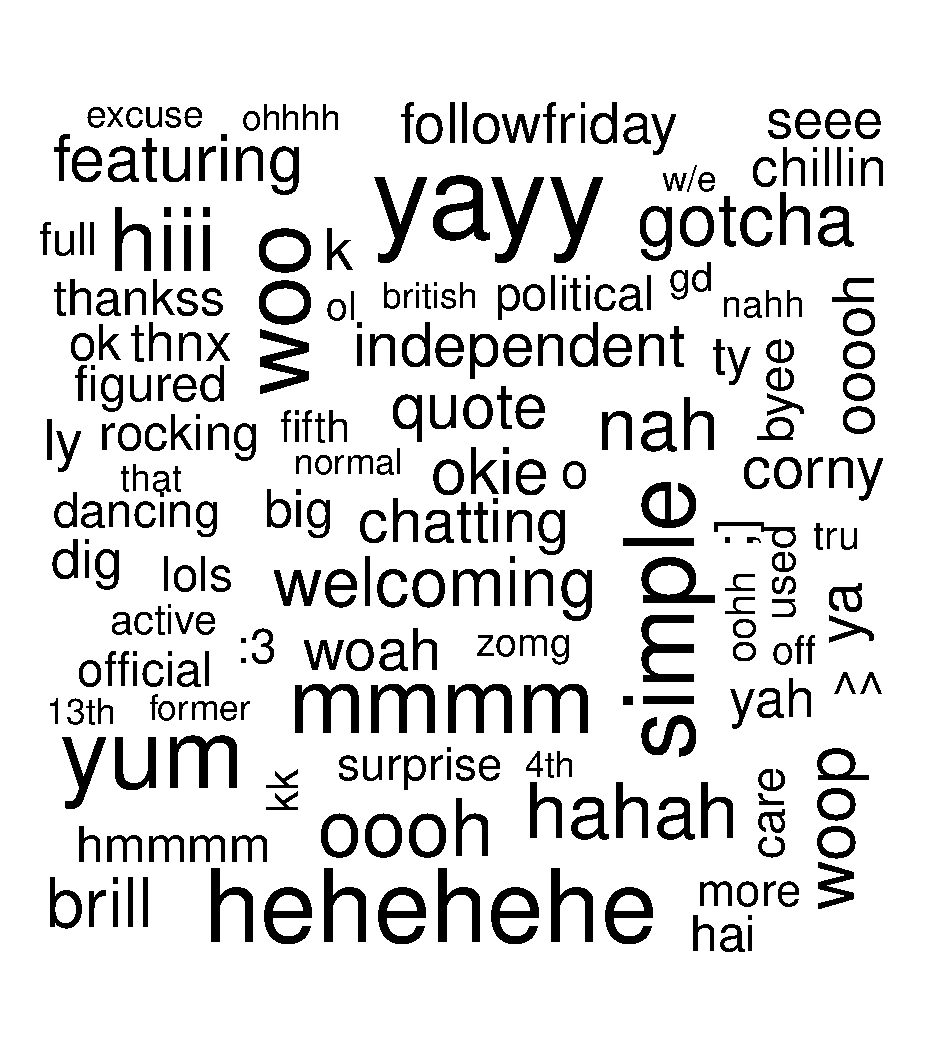
\includegraphics[scale=0.25]{../poswords.pdf}
&
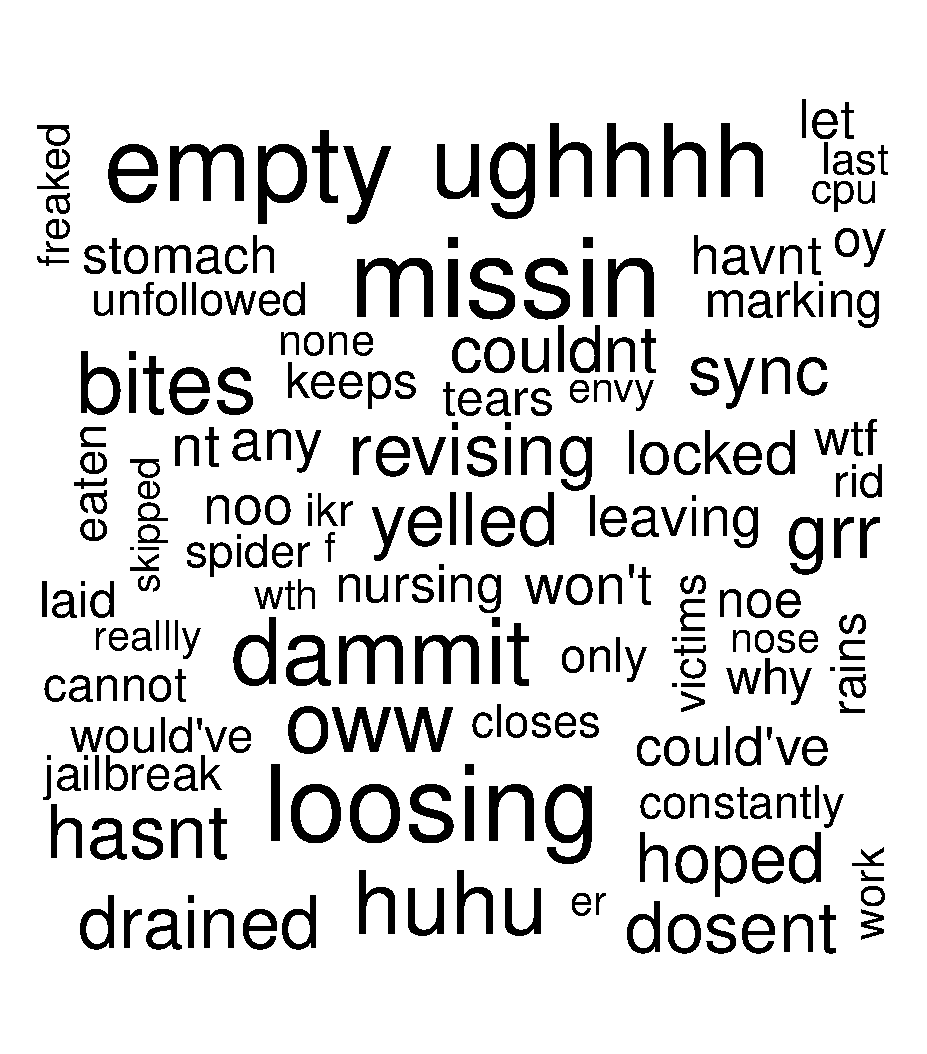
\includegraphics[scale=0.25]{../negwords.pdf}\\
(a) & (b)  
\end{tabular}
\caption{Word clouds of positive and negative words using log odds proportions.}
\label{fig:wordcloud}
\end{center}
\end{figure}
\end{frame}


\begin{frame}{Message-level classification}
\scriptsize
\begin{table}[htbp]
\begin{center}
\begin{tabular}{l|l|l|l|l}
\hline \hline
\multicolumn{ 5}{c}{Accuracy } \\ \hline \hline
Dataset & Baseline & ED & STS & Combination \\ \hline
6-coded & 71.79 $\pm$ 2.79 & 74.91 $\pm$ 2.56 $\circ$ & 75.11 $\pm$ 2.66 $\circ$ &  \textbf{75.31 $\pm$ 2.42} $\circ$ \\ 
Sanders & 71.43 $\pm$ 3.76 & 77.17 $\pm$ 3.68 $\circ$ & 77.32 $\pm$ 4.09 $\circ$ &  \textbf{77.54 $\pm$ 3.64} $\circ$ \\ 
SemEval & 76.81 $\pm$ 1.22 & 76.66 $\pm$ 1.38 & 77.7 $\pm$ 1.25 $\circ$ & \textbf{78.13 $\pm$ 1.38} $\circ$ \\ \hline \hline
\multicolumn{ 5}{c}{Weighted AUC } \\ \hline \hline
Dataset & Baseline & ED & S140 & Combination \\ \hline
6-coded & 0.77 $\pm$ 0.03 & 0.82 $\pm$ 0.03 $\circ$ & 0.82 $\pm$ 0.02 $\circ$ &  \textbf{0.83 $\pm$ 0.02} $\circ$ \\ 
Sanders & 0.77 $\pm$ 0.04 & 0.83 $\pm$ 0.04 $\circ$ & \textbf{0.84 $\pm$ 0.04} $\circ$  & \textbf{0.84 $\pm$ 0.04} $\circ$ \\ 
SemEval & 0.77 $\pm$ 0.02 & 0.81 $\pm$ 0.02 $\circ$ & \textbf{0.83 $\pm$ 0.02} $\circ$ &  \textbf{0.83 $\pm$ 0.02} $\circ$ \\ \hline
\end{tabular}
\caption{Message-level polarity classification performance.}
\label{tab:messclass}
\end{center}
\end{table}
\end{frame}


\begin{frame}{Discussions}
\begin{scriptsize}
\begin{itemize}
\item The method creates a lexicon with \textbf{disambiguated} POS entries and a probability distribution for \textbf{positive, negative, and neutral} classes. 
\item Sentiment analysis methods that are based on \textbf{SentiWordnet} can be easily adapted to \textbf{Twitter} by relying on our lexicon.
\item This method could be used to create \textbf{domain-specific} lexicons.
\item It could also be used to study the \textbf{dynamics} of opinion-words.
\item This method depends on a collection of \textbf{emoticon-annotated tweets}.
\item It would be hard to apply to \textbf{domains} where emoticons are not \textbf{frequently used}.

\end{itemize}
\end{scriptsize}

\end{frame}


\begin{frame}{Information Fusion Extension}

\begin{figure}[htb]
	\centering
	 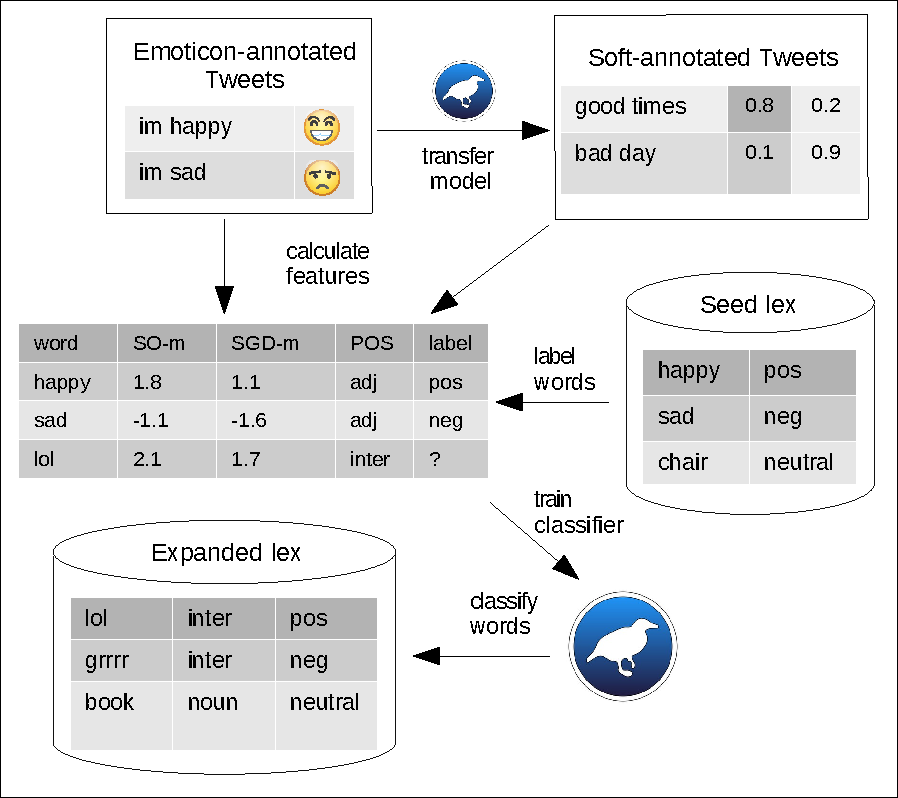
\includegraphics[scale=0.6]{infus.pdf}
\end{figure}



\end{frame}



\begin{frame}{Lexicon generation from unlabelled Tweets}
\begin{scriptsize}
\begin{itemize}
\item We propose another supervised model for lexicon expansion referred to as the \textbf{tweet-centroid model}.
\item The words are represented by \textbf{high-dimensional vectors} based on the context's where they occur. 
\item In contrast to the previous approach the expansion is done from \textbf{unlabelled tweets}.
\item It is inspired by the \textbf{Distributional Hypothesis} \cite{harris1954}: words occurring in the same \textbf{contexts} tend to have similar meanings.
\item Or equivalently: ``a word is characterized by the \textbf{company} it keeps".
\end{itemize}
\end{scriptsize}
\end{frame}


\begin{frame}{Lexicon generation from unlabelled Tweets (2)}
\begin{scriptsize}
\begin{itemize}
\item We treat a \textbf{whole tweet} as a word's context.
\item We model tweets as \textbf{vectors} calculated from the \textbf{content}.
\item We calculate word-level vectors based on the \textbf{centroids} of the \textbf{tweet-vectors} where a word occurs.
\item We suggest that words exhibiting a \textbf{certain polarity} are more likely used in contexts expressing the \textbf{same polarity} than in contexts exhibiting a \textbf{different one}. 
\end{itemize}
\end{scriptsize}
\end{frame}



\begin{frame}{Lexicon generation from unlabelled Tweets (3)}
\begin{scriptsize}
Tweets in the collection are represented by \textbf{two vectors}:
\begin{enumerate} 
\item A word-frequency \textbf{bag-of-words vector}. 
\item A semantic vector based on \textbf{word-clusters}. 
\end{enumerate}
\begin{figure}[ht]
	\centering
	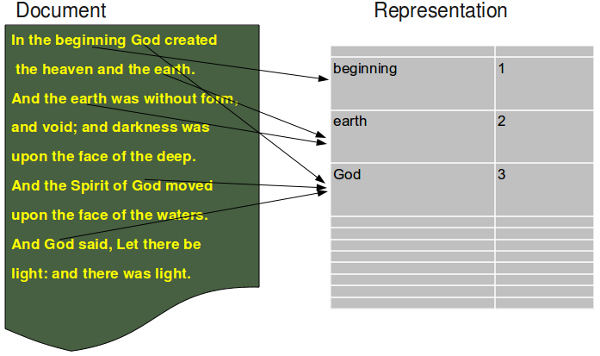
\includegraphics[scale=0.3]{pics/bow.png}
	\label{fig:word_clash}
\end{figure}

\end{scriptsize}
\end{frame}



\begin{frame}{Bag-of-words model}
\begin{scriptsize}
\begin{itemize}
\item Suppose we have a \textbf{corpus} $\mathcal{C}$ formed by $n$ tweets $t_1,\dots,t_n$.
\item  Each \textbf{tweet} \textbf{$t$} is a sequence of words.
\item  Let $\mathcal{V}$ be the \textbf{vocabulary} formed by the $m$ different words $w_1,$ $\dots, w_m$ found in $\mathcal{C}$.
\item  The tweet-level bag-of-words model represents each tweet $t$ as a \textbf{m-dimensional vector} $\overrightarrow{t}$.
\item Each dimension $\overrightarrow{t}_j$ corresponds to the \textbf{frequency} in which the word $w_j$ appears in $t$.   


\end{itemize}
\end{scriptsize}
\end{frame}



\begin{frame}{Bag-of-words model (2)}
\begin{scriptsize}
\begin{itemize}

\item We define the \textbf{word-tweet set} $\mathcal{W}(w)$ as the set of tweets in which $w$ is \textbf{observed}:
\begin{equation}
\mathcal{W}(w)=\{ t: w \in t, \forall t \in \mathcal{C}\}
\end{equation}

\item We define the word-level vector $\overrightarrow{w}$ as as the \textbf{centroid} of all tweet-vectors in which $w$ is used. 

\item $\overrightarrow{w}$ is a m-dimensional vector in which each dimension $w_j$ is calculated as follows:
\begin{equation}
\overrightarrow{w}_j = \sum_{t \in \mathcal{W}(w)} \frac{f_j(t)}{|\mathcal{W}(w)|}
\end{equation}

\item Bag-of-words models tend to produce \textbf{high dimensional sparse vectors}.

\end{itemize}
\end{scriptsize}
\end{frame}



\begin{frame}{Word-clusters model}
\begin{scriptsize}
\begin{itemize}

\item Let be $c$ a \textbf{clustering} functions that \textbf{maps} the $m$ words to a \textbf{partition} of the vocabulary $\mathcal{S}$ of $k$ classes, with $k \ll m$. 
\item This function is trained in an \textbf{unsupervised fashion} from a corpus of tweets using the \textbf{Brown clustering} algorithm \cite{brown1992class}. 
\item This algorithm produces \textbf{hierarchical clusters} by maximising the mutual information of \textbf{bigrams}.
\item These clusters have shown to be useful for tagging tweets according to \textbf{part-of-speech} classes \cite{twitterNLP}.
\end{itemize}
\end{scriptsize}
\end{frame}


\begin{frame}{Word-clusters model (2)}
\begin{scriptsize}
\begin{itemize}
\item We \textbf{tag} the word sequences of the tweets from $\mathcal{C}$ with the clustering function $c$.
\item We create a new \textbf{tweet-level} vector $\overrightarrow{tc}$ of $k$ dimensions based on the \textbf{frequency} of occurrence of a cluster $s$ in the tweet. 
\item We take the \textbf{centroids} of the cluster-based vectors $\overrightarrow{tc}$ from the tweets of $\mathcal{W}(w)$, producing $k$-dimensional word vectors.

\end{itemize}
\end{scriptsize}
\end{frame}

\begin{frame}{Tweet-centroid Model}

\begin{figure}[htb]
	\centering
	 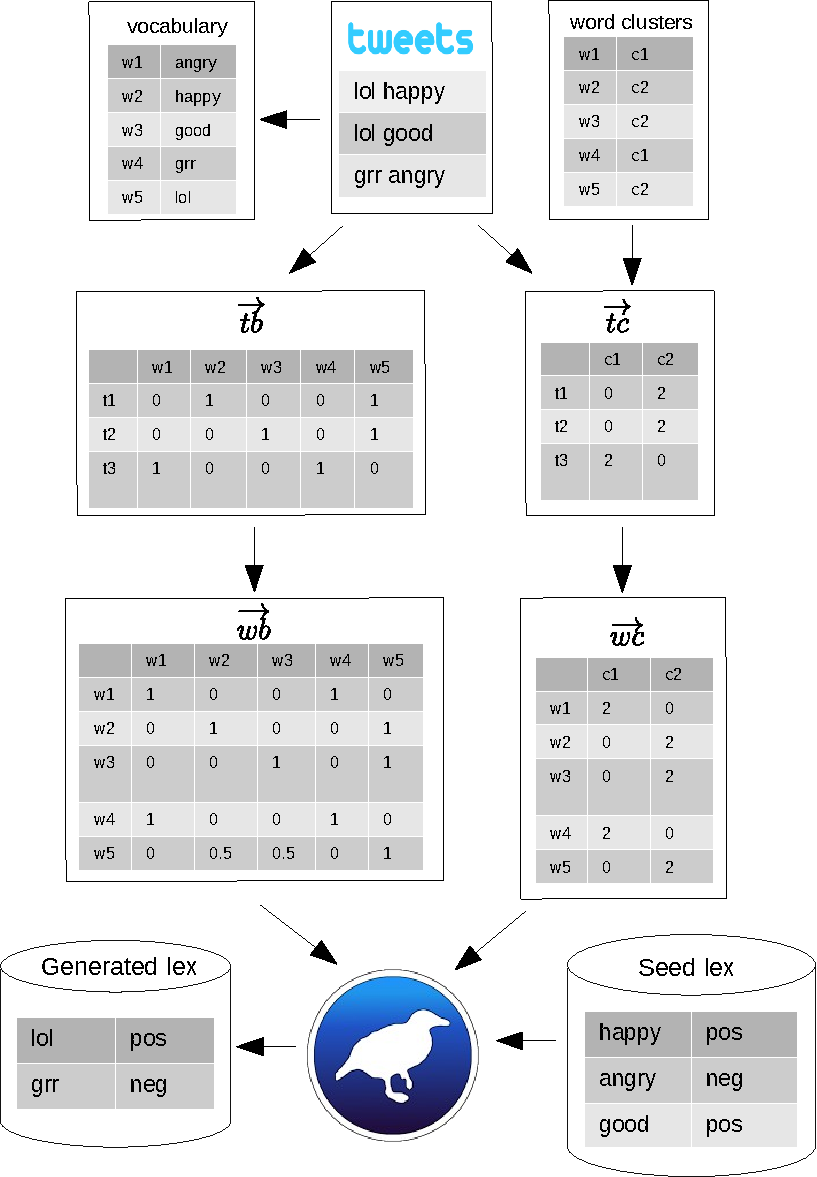
\includegraphics[scale=0.4]{sigirmodel.pdf}
\end{figure}



\end{frame}


\begin{frame}{Datasets}

\begin{scriptsize}
\begin{itemize}
\item We take a \textbf{random sample} of 2.5 million English tweets from the Edinburgh Corpus and STS.
\item  ED corpus represents a \textbf{realistic sample} from a stream of tweets.
\item  STS was \textbf{intentionally manipulated} to over-represent the presence of subjective tweets. 
\item We study these datasets to observe the effects of \textbf{manipulating} the collection of tweets for lexicon generation. 
\item We tokenise the tweets from both collections and create the word-level vectors $\overrightarrow{w}$ and $\overrightarrow{wc}$.
\end{itemize}
\end{scriptsize}

\begin{table}[htbp]
\scriptsize
\begin{center}
\begin{tabular}{ l|r|r}
\hline \hline
Dataset & \multicolumn{1}{c|}{STS} & \multicolumn{1}{c}{ED} \\ \hline 
\#tweets & $1,600,000$ & $2,500,000$ \\ 
\#positive words & $2015$ & $2639$ \\ 
\#negative words & $2621$ & $3642$ \\ 
\#neutral words & $3935$ & $5085$ \\ 
\#unlabelled words & $36,451$ & $67,692$ \\ 
\#bag-of-words attributes & $45,022$ & $79,058$ \\ 
\#cluster-vector attributes & $993$ & $999$ \\ \hline \hline
\end{tabular}
\end{center}
\label{tab:corpstats}
\end{table}
\end{frame}



\begin{frame}{Word-level 2-class polarity classification performance}
\begin{scriptsize}
\begin{table}[!htb]
\scriptsize
\begin{center}
\begin{tabular}{l|c|c|c}
\hline \hline
\multicolumn{ 4}{c}{Accuracy } \\ \hline \hline
Dataset & WORDS & CLUSTER & ALL \\ \hline
%ED EM & 76.62 $\pm$ 1.75 & 77.29 $\pm$ 1.69 & \textbf{78.35 $\pm$ 1.84} $\circ$ \\ 
STS & 75.52 $\pm$ 1.81 & 77.2 $\pm$ 1.9 $\circ$ & \textbf{77.85 $\pm$ 1.94} $\circ$ \\ 
ED  & 77.75 $\pm$ 1.54 & 77.62 $\pm$ 1.37 & \textbf{79.15 $\pm$ 1.39} $\circ$ \\ 
\hline \hline
\multicolumn{ 4}{c}{AUC} \\ \hline \hline
Dataset & WORDS & CLUSTER & ALL \\ \hline
%ED EM & 0.85 $\pm$ 0.02 & 0.85 $\pm$ 0.02 & \textbf{0.86 $\pm$ 0.02} $\circ$ \\
STS & 0.83 $\pm$ 0.02 & 0.84 $\pm$ 0.02 $\circ$ & \textbf{0.85 $\pm$ 0.02} $\circ$ \\
ED  & 0.85 $\pm$ 0.01 & 0.85 $\pm$ 0.01 & \textbf{0.86 $\pm$ 0.01} $\circ$ \\ 
 \hline
\end{tabular}
\end{center}
\end{table}
\end{scriptsize}
\end{frame}

\begin{frame}{Word-level 3-class polarity classification performance}
\begin{scriptsize}
\begin{table}[!htb]
\scriptsize
\begin{center}
\begin{tabular}{l|c|c|c}
\hline \hline
\multicolumn{ 4}{c}{Accuracy } \\ \hline \hline
Dataset & WORDS & CLUSTER & ALL \\ \hline
%ED EM & 62.96 $\pm$ 1.43 & 64.22 $\pm$ 1.24  $\circ$ & \textbf{65.02 $\pm$ 1.3} $\circ$ \\ 
STS & 61.84 $\pm$ 1.46 & 64.42 $\pm$ 1.54 $\circ$ & \textbf{64.57 $\pm$ 1.44} $\circ$ \\
ED  & 62.93 $\pm$ 1.31 & 64.5 $\pm$ 1.16 $\circ$ & \textbf{65.5 $\pm$ 1.19} $\circ$ \\ 
 \hline \hline
\multicolumn{ 4}{c}{AUC} \\ \hline \hline
Dataset & WORDS & CLUSTER & ALL \\ \hline
%ED EM & 0.77 $\pm$ 0.01 & \textbf{0.79 $\pm$ 0.01} $\circ$ & \textbf{0.79 $\pm$ 0.01} $\circ$ \\
STS & 0.77 $\pm$ 0.01 & \textbf{0.79 $\pm$ 0.01} $\circ$ & \textbf{0.79 $\pm$ 0.01} $\circ$ \\ 
ED  & 0.78 $\pm$ 0.01 & 0.79 $\pm$ 0.01 $\circ$ & \textbf{0.8 $\pm$ 0.01} $\circ$ \\ 
\hline
\end{tabular}
\end{center}
\end{table}
\end{scriptsize}
\end{frame}


\begin{frame}{Generated words example}
\begin{scriptsize}
 \begin{table}[htbp]
 \scriptsize
\begin{center}
\begin{tabular}{l|l|c|c|c}
\hline
\multicolumn{1}{c|}{word} & \multicolumn{1}{c|}{label} & negative & neutral & positive \\ \hline
\#recession & negative & 0.603 & 0.355 & 0.042 \\ 
\#silicon\_valley & neutral & 0.043 & 0.609 & 0.348 \\ 
bestfriends & positive & 0.225 & 0.298 & 0.477 \\ 
christamas & positive & 0.003 & 0.245 & 0.751 \\ 
comercials & negative & 0.678 & 0.317 & 0.005 \\ 
hhahaha & positive & 0.112 & 0.409 & 0.479 \\ 
powerpoint & neutral & 0.068 & 0.802 & 0.13 \\ 
psychotic & negative & 0.838 & 0.138 & 0.024 \\ 
widows & negative & 0.464 & 0.261 & 0.275 \\ 
yassss & positive & 0.396 & 0.08 & 0.524 \\ \hline
\end{tabular}
\end{center}
\end{table}
\end{scriptsize}
\end{frame}




\begin{frame}{Message-level classification performance}
\begin{scriptsize}
 \begin{table}[htbp]
\scriptsize
\begin{center}
\begin{tabular}{l|c|c|c}
\hline \hline
\multicolumn{ 4}{c}{Accuracy } \\ \hline \hline
Dataset & Baseline & STS & ED \\ \hline
Sanders & 73.25 $\pm$ 3.51 & 74.76 $\pm$ 4.21 & \textbf{76.58 $\pm$ 3.8} $\circ$ \\ 
6-human & 72.84 $\pm$ 2.57 & 75.08 $\pm$ 2.31 $\circ$ & \textbf{76.42 $\pm$ 2.34} $\circ$ \\ 
SemEval & 77.72 $\pm$ 1.24 & 78.97 $\pm$ 1.31 $\circ$ & \textbf{79.18 $\pm$ 1.22} $\circ$ \\ \hline \hline
\multicolumn{ 4}{c}{AUC} \\ \hline \hline
Dataset & Baseline & STS & ED \\ \hline
Sanders & 0.78 $\pm$ 0.04 & 0.8 $\pm$ 0.04 $\circ$ & \textbf{0.83 $\pm$ 0.04} $\circ$ \\ 
6-human & 0.79 $\pm$ 0.03 & 0.82 $\pm$ 0.03 $\circ$ & \textbf{0.83 $\pm$ 0.02} $\circ$ \\ 
SemEval & 0.78 $\pm$ 0.02 & 0.82 $\pm$ 0.02 $\circ$ & \textbf{0.84 $\pm$ 0.02} $\circ$ \\ \hline
\end{tabular}
\end{center}
\end{table}
\end{scriptsize}
\end{frame}







\begin{frame}{Discussions}
\begin{scriptsize}
\begin{itemize}
\item  Collections of tweets manipulated to over-represent subjective tweets are not necessarily \textbf{better} for lexicon generation than random collections of tweets.
\item The proposed technique relies on resources that are relatively \textbf{cheap} to obtain: a \textbf{seed lexicon}, and a collection of \textbf{unlabelled tweets}.
\item Source code available: \url{http://www.cs.waikato.ac.nz/ml/sa/lex.html}.
\end{itemize}
\end{scriptsize}
\end{frame}


\begin{frame}{Comparison of both models}
\begin{scriptsize}
\begin{table}[htbp]
\begin{center}
\begin{tabular}{l|l|l}
\hline
 & Time-series & Tweet-Centroid \\ \hline
Depends on a seed lexicon & Yes & Yes \\ 
Detects neutral words & Yes & Yes \\ 
Depends on labelled tweets & Yes & No \\ 
Dimensionality & Low & High \\ 
POS disambiguation & Yes & No \\ 
Considers time & Yes & No \\ 
Suitable for stream learning & Yes & Yes \\ 
Suitable for emotion detection & No & Yes \\ \hline
\end{tabular}
\end{center}
\end{table}
\end{scriptsize}
\end{frame}







\begin{frame}{Future Work}
\begin{scriptsize}
\begin{itemize}
\item Use the Tweet-centroid model for \textbf{emotion} classification using \textbf{multi-label classification}.
\item Transfer other message-level attributes to the word-level, e.g., n-grams, POS-tags.
\item Design a mechanism to discover opinion words in an \textbf{online fashion}.
\end{itemize}




\end{scriptsize}
\end{frame}





\begin{frame}
\frametitle{Questions?}
%\vspace{1.5cm}
\begin{center}\LARGE Thanks for your Attention!\\ \end{center}

\begin{columns}
\begin{column}{0.55\textwidth}
\begin{block}{Acknowledgments}
\begin{itemize}\tiny
	\item University of Waikato Doctoral Scholarship
	\item Machine Learning Group at the University of Waikato
	
\end{itemize}
\end{block}
\end{column}
\begin{column}{0.45\textwidth}
\vspace{1.5cm}

\begin{figure}[h!]
	\centering
	\includegraphics[scale=0.3]{../../img/waikato.png}
\end{figure}
\end{column}
\end{columns}

\end{frame}

\begin{frame}[allowframebreaks]\scriptsize
\frametitle{References}
\bibliography{../bio}
\bibliographystyle{apalike}
%\bibliographystyle{flexbib}
\end{frame}  


%%%%%%%%%%%%%%%%%%%%%%%%%%%

\end{document}
